\documentclass[../report.tex]{subfiles}

\begin{document}
В данном разделе сравниваются реализованные алгоритмы, дается сравнительная оценка затрат на время.

\section{Пример работы программы}
Пример работы программы представлен на рисунке \ref{fig:ex}.
\captionsetup{singlelinecheck=true}
\begin{figure}[H]
	\centering
	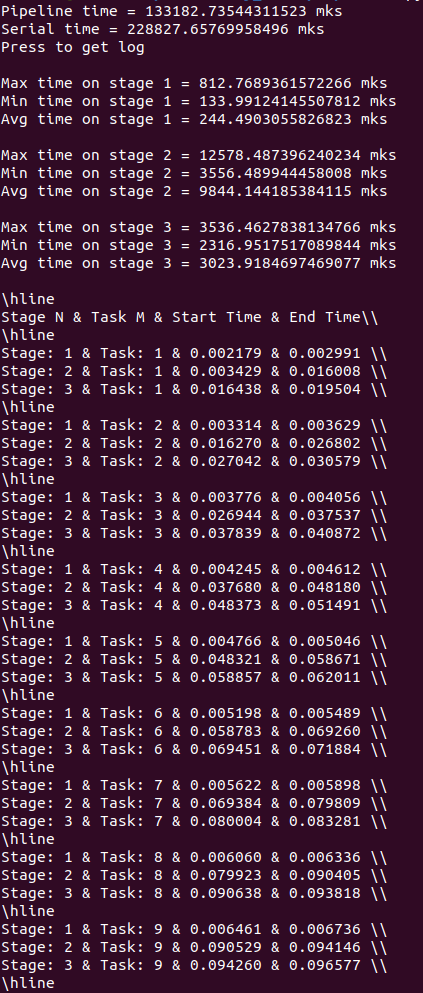
\includegraphics[width=0.62\linewidth]{images/example}
	\caption{Пример работы программы}
	\label{fig:ex}
\end{figure}

\section{Технические характеристики}
Технические характеристики устройства, на котором выполнялось исследование:
\begin{itemize}
	\item операционная система: Fedora 35 ~\cite{os};
	\item оперативная память: 16 Гб;
	\item процессор: AMD Ryzen5 2500U~\cite{processor}:
	\begin{itemize}
		\item количество физических ядер: 4;
		\item количество логических ядер: 8.
	\end{itemize}
\end{itemize}

\section{Время выполнения алгоритмов}
Время выполнения алгоритмов измерялось на автоматически генерируемых в необходимом количестве пользовательских данных с использованием функции time библиотеки time. Замеры производились на компьютере, подключенном к сети электропинания с отключенным режимом энергосбережения. Усредненные результаты 10 замеров реального времени работы приведены в таблице ниже.

На рисунке \ref{fig:graph} представлена зависимость времени выполнения алгоритма в зависимости от <<плана на день>> -- количества пользователей для обработки - на основе таблицы \ref{tab:time}. Последовательное выполнение занимает в среднем в 1.5-1.7 раз больше времени, чем конвейерное с незначительным увеличением выигрыша обработки на конвейере при увеличении количества пользователей. Таким образом, выигрыш от использования конвейерной обработки при количестве пользователей от 15 до 85 приблизительно одинаков и составляет около 1.6 раз.
\begin{table}[H]
	\begin{center}
		\captionsetup{justification=raggedleft, singlelinecheck=false}
		\caption{\label{tab:time} Время выполнения алгоритма для разного количества пользователей в микросекундах}
		\begin{tabular}{|c| c | c|} 
			\hline
			Размер&Последовательное выполнение&Конвейерная обработка\\ [0.5ex]
			\hline
			5 &   38291.287 &  36348.152\\ 
			\hline
			15 &   109756.374 &   73250.5798 \\ 
			\hline
			25 &   181147.265 &   113172.388 \\ 
			\hline
			35 &   252654.957 &   152421.474 \\ 
			\hline
			45 &  322310.686 &  197659.373 \\ 
			\hline
			55 & 399007.916 & 239235.663 \\ 
			\hline
			65 & 461043.334 & 286625.170 \\ 
			\hline
			75 & 541337.20 & 321961.14 \\ 
			\hline
		\end{tabular}
	\end{center}
\end{table}

\begin{figure}[H]
	\centering
	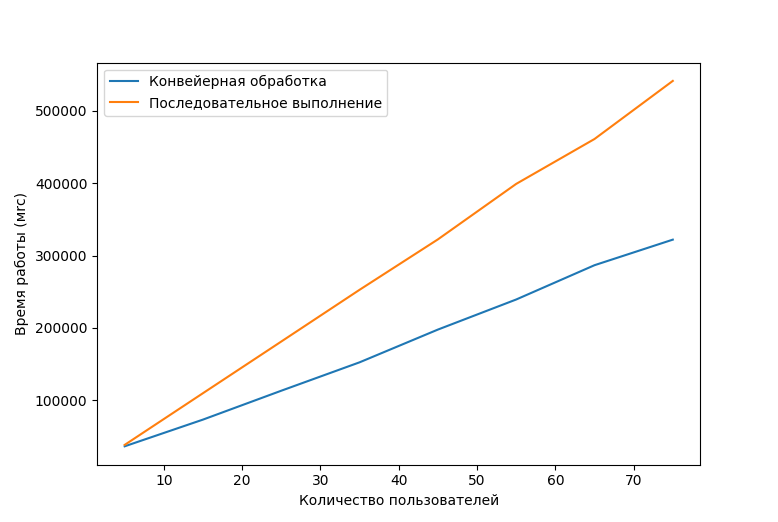
\includegraphics[width=0.9\linewidth]{images/con_vs_serial}
	\caption{Зависимость времени выполнения от количества пользователей}
	\label{fig:graph}
\end{figure}

\section{Тестирование}
Для тестирования корректности работы ПО используется анализ логов. Полученная для последних 6 заявок таблица приведена ниже. На рисунке \ref{fig:maxmintime} представлены данные о максимальном, минимальном и среднем времени обработки заявок на каждой ленте конвейера.
%
\begin{table}[H]
	\begin{center}
		\captionsetup{justification=raggedleft, singlelinecheck=false}
		\caption[]{\label{tab:tests} Полученный лог}
		%
		\begin{tabular}{|c|c|c|c|}
			\hline
			Stage N & Task M & Start Time & End Time\\
			\hline
			Stage: 1 & Task: 24 & 0.012759 & 0.012983 \\
			Stage: 2 & Task: 24 & 0.096859 & 0.100533 \\
			Stage: 3 & Task: 24 & 0.100766 & 0.103546 \\
			\hline
			Stage: 1 & Task: 25 & 0.013081 & 0.013289 \\
			Stage: 2 & Task: 25 & 0.100624 & 0.104318 \\
			Stage: 3 & Task: 25 & 0.104567 & 0.107468 \\
			\hline
			Stage: 1 & Task: 26 & 0.013381 & 0.013590 \\
			Stage: 2 & Task: 26 & 0.104418 & 0.108121 \\
			Stage: 3 & Task: 26 & 0.108363 & 0.111242 \\
			\hline
			Stage: 1 & Task: 27 & 0.013669 & 0.017236 \\
			Stage: 2 & Task: 27 & 0.108238 & 0.111867 \\
			Stage: 3 & Task: 27 & 0.112061 & 0.114830 \\
			\hline
			Stage: 1 & Task: 28 & 0.017447 & 0.017701 \\
			Stage: 2 & Task: 28 & 0.111984 & 0.115609 \\
			Stage: 3 & Task: 28 & 0.115740 & 0.118498 \\
			\hline
			Stage: 1 & Task: 29 & 0.017766 & 0.017931 \\
			Stage: 2 & Task: 29 & 0.115671 & 0.119328 \\
			Stage: 3 & Task: 29 & 0.119419 & 0.122284 \\
			\hline
			Stage: 1 & Task: 30 & 0.017987 & 0.018134 \\
			Stage: 2 & Task: 30 & 0.119397 & 0.123048 \\
			Stage: 3 & Task: 30 & 0.123159 & 0.126240 \\
			\hline
		\end{tabular}
	\end{center}
\end{table}
\captionsetup{singlelinecheck=true}
\begin{figure}[H]
	\centering
	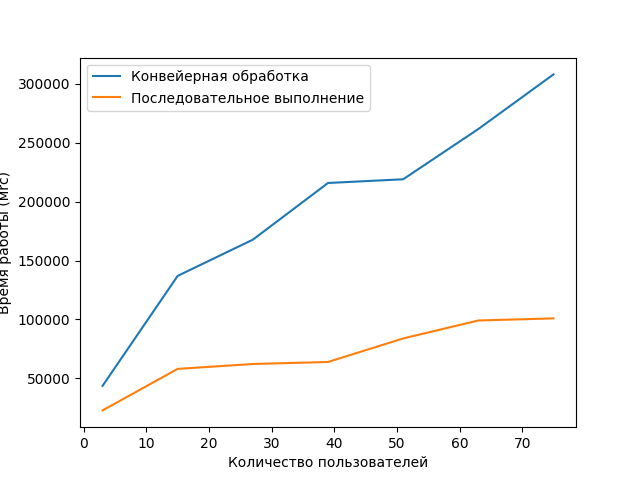
\includegraphics[width=0.65\linewidth]{images/maxmintime}
	\caption{Время выполнения заявок на каждой из лент конвейера}
	\label{fig:maxmintime}
\end{figure}


\section*{Вывод}
В данном разделе были проведены измерения времени, затрачиваемого на загрузку данных о пользователе из базы данных, хеширование пароля и сохранения в базу данных полученного хэша.
Для размера входной очереди конвейера, принадлежащего интервалу [5, 85], выигрыш по сравнению с последовательной обработкой составил приблизительно 1.5-1.7 раз с небольшими колебаниями при увеличении количества пользователей.
\newpage

\end{document}